\documentclass[border=6pt]{standalone}
\usepackage{amsmath}
\usepackage{tikz}
\usetikzlibrary{arrows.meta}
\begin{document}
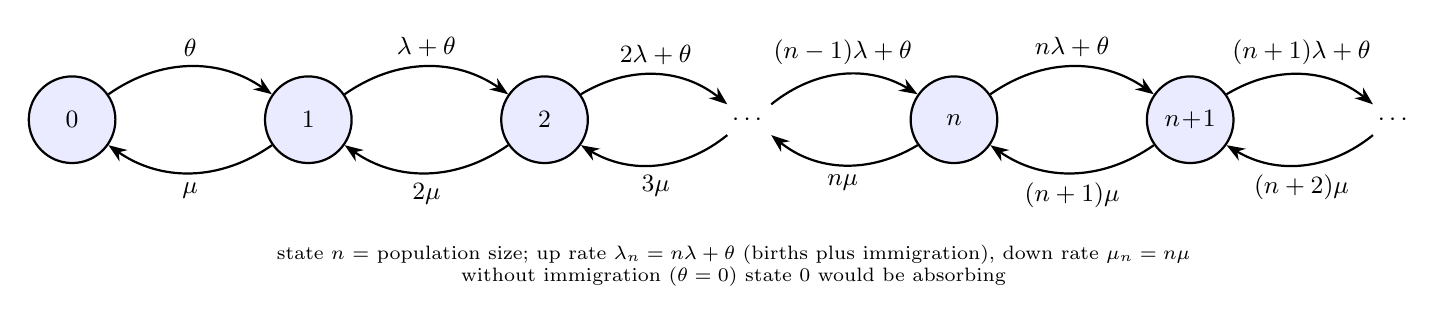
\begin{tikzpicture}[>=Stealth,font=\small,
 s/.style={draw,thick,circle,minimum size=1.1cm,inner sep=0pt,fill=blue!8},
 e/.style={->,thick},
 lab/.style={font=\small,fill=white,inner sep=1.5pt},
 every loop/.style={->,thick,looseness=6}]
\node[s] (0) at (0,0) {$0$};
\node[s] (1) at (3,0) {$1$};
\node[s] (2) at (6,0) {$2$};
\node (d) at (8.6,0) {$\cdots$};
\node[s] (n) at (11.2,0) {$n$};
\node[s] (n1) at (14.2,0) {$n\!+\!1$};
\node (d2) at (16.8,0) {$\cdots$};
\foreach \a/\b/\u/\v in {0/1/\theta/\mu,1/2/\lambda+\theta/2\mu,2/d/2\lambda+\theta/3\mu,d/n/(n-1)\lambda+\theta/n\mu,n/n1/n\lambda+\theta/(n+1)\mu,n1/d2/(n+1)\lambda+\theta/(n+2)\mu} {
  \draw[e] (\a) to[bend left=35] node[above]{$\u$} (\b);
  \draw[e] (\b) to[bend left=35] node[below]{$\v$} (\a);
}
\node[font=\scriptsize,align=center] at (8.4,-1.85) {state $n$ = population size; up rate $\lambda_n=n\lambda+\theta$ (births plus immigration), down rate $\mu_n=n\mu$\\without immigration ($\theta=0$) state 0 would be absorbing};
\end{tikzpicture}
\end{document}
